\documentclass[english,11pt,table,handout]{beamer}

\input{ipcv-style.tex}
\usepackage{pgf}

\newcommand{\Rule}[2]{\genfrac{}{}{0.7pt}{}{{\setlength{\fboxrule}{0pt}\setlength{\fboxsep}{3mm}\fbox{$#1$}}}{{\setlength{\fboxrule}{0pt}\setlength{\fboxsep}{3mm}\fbox{$#2$}}}}

\newcommand{\Rulee}[3]{\genfrac{}{}{0.7pt}{}{{\setlength{\fboxrule}{0pt}\setlength{\fboxsep}{3mm}\fbox{$#1$}}}{{\setlength{\fboxrule}{0pt}\setlength{\fboxsep}{3mm}\fbox{$#2$}}}[#3]}

\usepackage{url}

\usepackage{qtree}

\usepackage{datetime}

\usepackage{amsfonts}
\usepackage{mathtools}
\usepackage{fancybox}
\usepackage[linesnumbered]{algorithm2e}
\usepackage{ragged2e}
\usepackage{verbatim}



\usepackage{pgfplots}


\lecture[2]{Point Processing and Histogram}{lecture-text}

% \subtitle{Sequence Control}

\date{August 15, 2018}
\newcounter{saveenumi}

\usepackage{wrapfig}
\usetikzlibrary{automata,arrows,positioning, chains, shapes.callouts, calc}

\tikzstyle{mnode}=[circle, draw, fill=black, inner sep=0pt, minimum width=4pt]
\tikzstyle{thinking} = [draw=blue, very thick]
\edef\sizetape{1cm}
\tikzstyle{tmtape}=[draw,minimum size=\sizetape]
\tikzstyle{tmhead}=[arrow box,draw,minimum size=.5cm,arrow box
arrows={east:.25cm, west:0.25cm}]
\tikzset{
  level/.style   = { ultra thick, blue },
  connect/.style = { dashed, red },
  notice/.style  = { draw, rectangle callout, callout relative pointer={#1} },
  label/.style   = { text width=4cm }
}

\begin{document}

\begin{frame}
\selectlanguage{english}
  \maketitle
\end{frame}

\begin{frame}\frametitle<presentation>{Overview}
  \tableofcontents
\end{frame}

%%%%%%%%%%%%%%%%%%%%%%%%%%%%%%%%%%%%%%%%%%%%%%%%%%%%%%%%%%%%%%%%%%%%%
%%%%%%%%%%%%%%%%%%%%%%%%%%%%%%%%%%%%%%%%%%%%%%%%%%%%%%%%%%%%%%%%%%%%%


%\frame
%{
%	\Huge
%	\begin{center}
%	\textcolor{blue}{\textbf{What is local processing?}}
%	\end{center}
%}

\section{Point processing}
\frame
{
	\frametitle{Point processing}
	\selectlanguage{english}
	\begin{block}{Concepts}
		\begin{itemize}
			\item Image: $f(x,y)$
			\begin{enumerate}
				\item $x$: discrete variable, in $[0,1, .., N]$
				\item $y$: discrete variable, in $[0,1, .., M]$
				\item $f(x,y)$: discrete value, in $[0,1, .., 255]$
			\end{enumerate}
			\item point $\equiv$ pixel
			\item $f(x,y)$: has $M \times N$ points (or pixels)
		\end{itemize}
	\end{block}

	
}
\frame
{
	\frametitle{Point processing}
	\selectlanguage{english}
	\begin{block}{Definition and Notation}
		\begin{itemize}
			\item \textbf{Point processing}: Process each point by a function that depends ONLY the pixel's value and that does not depend on the point's neighbors.	
			\item Pixel processing function:
			\begin{itemize}
				\item referred to as \textbf{transfer function}
				\item denoted as $T[.]$
			\end{itemize} 
		\end{itemize}
	\end{block}

	\begin{figure}[!h]
		\begin{tabular}{cc}
			\includegraphics[scale=0.4]{point_process_model.png} &
		\end{tabular}
		
	\end{figure}
	\begin{itemize}
		\item $f(x,y)$: input image
		\item $g(x,y) = T[f(x,y)]$: output image
	\end{itemize}
	
}

\subsection{Linear transformation}
\begin{frame}[fragile]
	\frametitle{Point processing}
	\selectlanguage{english}
	\begin{block}{Linear transformation: Math}
		\begin{itemize}
			\item  $g(x,y) = a \times f(x,y) + b$
			\item Where, $a$ and $b$: pre-defined parameters
		\end{itemize}
	\end{block}

	\begin{block}{Linear transformation: Applications}
		\begin{itemize}
			\item General: Change the image's intensity, cause the input bighter or darker
			\begin{itemize}
				\item Users have to choose appropriate $a$ and $b$ (manually)
			\end{itemize}
			\item Specific:
			\begin{itemize}
				\item Create negative images
				\item Convert to back-white image
			\end{itemize}
		\end{itemize}
	\end{block}
\end{frame}

\begin{frame}[fragile]
\frametitle{Point processing}
\selectlanguage{english}
\begin{block}{Linear transformation: with Matlab}
	\lstset{language=Matlab, basicstyle=\small, escapeinside={\%*}{*)}}
	\begin{lstlisting}
	%read input image
	im = imread('cameraman.tif');
	%set parameters
	a1 = 1.5; b1 = 20;
	a2 = 1.5; b2 = 50;
	a3 = 0.5; b3 = 0;
	%transform the input
	im1 = a1 * im  + b1; %clipped to [0,255] auto
	im2 = a2 * im  + b2; %clipped to [0,255] auto
	im3 = a3 * im  + b3; %clipped to [0,255] auto
	
	
	\end{lstlisting}
\end{block}
\end{frame}

\begin{frame}[fragile]
\frametitle{Point processing}
\selectlanguage{english}
\begin{block}{Linear transformation: with Matlab(continued)}
	\lstset{language=Matlab, basicstyle=\tiny, escapeinside={\%*}{*)}}
	\begin{lstlisting}
	%show output image
	figure;
	subplot(2,2,1); imshow(im); title('input image')
	subplot(2,2,2); imshow(im1); 
	t1 = sprintf('output image [a =%5.2f, b = %5.2f]',
	              a1, b1); 
	title(t1)
	subplot(2,2,3); imshow(im2); 
	t2 = sprintf('output image [a =%5.2f, b = %5.2f]', 
	              a2, b2); 
	title(t2)
	subplot(2,2,4); imshow(im3); 
	t3 = sprintf('output image [a =%5.2f, b = %5.2f]', 
	              a3, b3); 
	title(t3)
	suptitle('Linear Transformation: output =  a*input + b');	
	\end{lstlisting}
\end{block}
\end{frame}

\begin{frame}[fragile]
	\frametitle{Point processing}
	\selectlanguage{english}
	\begin{block}{Linear transformation: Illustration}
	\begin{figure}[!h]
		\begin{table}
		\begin{tabular}{cc}
			\includegraphics[width=2.3cm]{./images/cameraman.png} & \includegraphics[width=2.3cm]{./images/cameraman1.png} \\
			Input image & Output Image \\
			 & $[a=1.5, b=20]$ \\
			\includegraphics[width=2.3cm]{./images/cameraman2.png} &
			 \includegraphics[width=2.3cm]{./images/cameraman3.png} \\
			 Output Image  & Output Image \\
			 $[a=1.5, b=50]$ & $[a=0.5, b=0]$ 
			 
		\end{tabular}
		\caption{Linear Transformation: \textbf{output} = a * \textbf{input} + b}
		\end{table}
	\end{figure}	
	\end{block}
\end{frame}

\begin{frame}[fragile]
\frametitle{Point processing}
\selectlanguage{english}
\begin{block}{Linear transformation: Illustration}
	\begin{figure}[!h]
		\begin{table}
			\begin{tabular}{c}
				\includegraphics[width=7cm]{./images/linear_negative.png}
				
			\end{tabular}
			\caption{Creating negative image: \textbf{output} = a * \textbf{input} + b; where, $\mathbf{a=-1, b = 255}$}
		\end{table}
	\end{figure}	
\end{block}
\end{frame}


\begin{frame}[fragile]
\frametitle{Point processing}
\selectlanguage{english}
\begin{block}{Linear transformation: Illustration}
	\begin{figure}[!h]
		\begin{table}
			\begin{tabular}{c}
				\includegraphics[height=6.5cm]{./images/negative_demo.png}
				
			\end{tabular}
			\caption{Creating negative image: \textbf{output} = a * \textbf{input} + b; where, $\mathbf{a=-1, b = 255}$}
		\end{table}
	\end{figure}	
\end{block}
\end{frame}

\subsection{Logarithmic transformation}
\begin{frame}[fragile]
\frametitle{Point processing}
\selectlanguage{english}
\begin{block}{Logarithmic transformation: Math}
	\begin{itemize}
		\item  $g(x,y) = a \times \log[{1 + f(x,y)] + b}$
		\item Where, $a$: a pre-defined parameter
	\end{itemize}
\end{block}

\begin{block}{Logarithm function}
	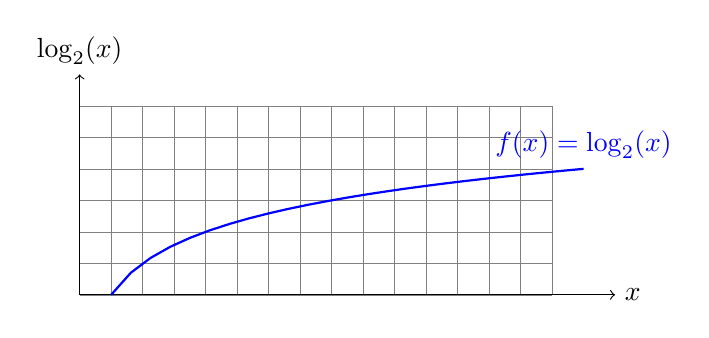
\begin{tikzpicture}[scale=0.4,domain=1:16]
	\draw[very thin,color=gray] (0,0) grid (15,6);
	% Draw axes
	\draw [<->] (0,7) node (yaxis) [above] {$\log_2(x)$}
	|- (17,0) node (xaxis) [right] {$x$};
	
	\draw[color=blue, thick] plot (\x,{log2(\x)})
	node[above] {$f(x) = \log_2(x)$};
	
	%\draw[color=blue, dashed] (0,0) -- (15,15) node[above] {$f(n)=n$};
	%\draw[color=blue, dashed] (0,0) -- (16, 8) node[above] {$f(n)=n/2$};
	\end{tikzpicture}
	
	\begin{itemize}
		\item a large value $(x)$ $\rightarrow$ mapped to a smaller value $(\log_2 x)$
		\item a large distance between two intensities in the input image $\rightarrow$ mapped to a smaller distance in the output image
	\end{itemize}
\end{block}
\end{frame}

\begin{frame}[fragile]
\frametitle{Point processing}
\selectlanguage{english}

\begin{block}{Logarithmic transformation: Applications}
	\begin{itemize}
		\item Input image: 
		\begin{itemize}
			\item have some regions with too dark intensities (\textbf{near 0})
			\item have some regions with too bright intensities (\textbf{near 255})
		\end{itemize}
	
		\item Requirement:
		\begin{itemize}
			\item Make dark regions brighter while keeping the intensity in bright regions lower than 255.
			\item Or, make bright regions darker while keeping the intensity in dark regions lower than 0.
		\end{itemize}
		\item Solution: use logarithmic transformation
		\item Often case:
		\begin{itemize}
			\item Should use logarithmic transformation to enhance the result of FFT before displaying
		\end{itemize}
			
	\end{itemize}
\end{block}
\end{frame}



\begin{frame}[fragile]
\frametitle{Point processing}
\selectlanguage{english}
\begin{block}{Logarithmic transformation: Illustration}
	\begin{figure}[!h]
		\begin{table}
			\begin{tabular}{c}
				\includegraphics[height=6.5cm]{./images/log_trans.png}
				
			\end{tabular}
			\caption{Samples}
		\end{table}
	\end{figure}	
\end{block}
\end{frame}



\subsection{Exponential transformation}
\begin{frame}[fragile]
\frametitle{Point processing}
\selectlanguage{english}
\begin{block}{(Inverse-log) Exponential transformation: Math}
	\begin{itemize}
		\item  $g(x,y) = a \times e^{f(x,y)} + b$
		\item Where, $a$  and $b$: pre-defined parameters
	\end{itemize}
\end{block}

\begin{block}{Exponential function}
	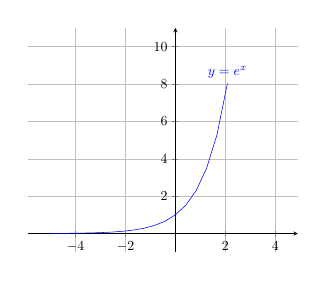
\begin{tikzpicture}[scale=0.5]
		\begin{axis}[grid=both,
				xmax=4,ymax=10,
				axis lines=middle,
				restrict y to domain=-1:10,
				enlargelimits]
		\addplot[blue]  {pow(e,x)} node[above]{$y=e^x$};
		\end{axis}
	\end{tikzpicture}
	
	\begin{itemize}
		\item a small value $(x)$ $\rightarrow$ mapped to a larger value $e^x$
		\item a small distance between two intensities in the input $\rightarrow$ mapped to a larger distance in the output image
	\end{itemize}
\end{block}
\end{frame}


\begin{frame}[fragile]
\frametitle{Point processing}
\selectlanguage{english}

\begin{block}{Exponential transformation: Applications}
	\begin{itemize}
		\item map small differences between two intensities in the input to a larger differences in the output image (\textbf{contrast input images	})
	\end{itemize}
\end{block}

\begin{block}{Exponential transformation: with Matlab}
	\lstset{language=Matlab, basicstyle=\small, escapeinside={\%*}{*)}}
	\begin{lstlisting}
	%read input image
	path = 'coffebean.png'
	im = imread(path); %range [0->255]
	%convert double image: [0->1]
	im = im2double(im);
	%set parameters
	a = 1; b = -1;
	%transform input image
	im1 = a * exp(im) + b;
	%normalize the output, to [0->1]
	im1 = im1./max(im1(:));
	\end{lstlisting}
\end{block}
\end{frame}

\begin{frame}[fragile]
\frametitle{Point processing}
\selectlanguage{english}

\begin{block}{Exponential transformation: with Matlab (continued)}
	\lstset{language=Matlab, basicstyle=\small, escapeinside={\%*}{*)}}
	\begin{lstlisting}
	%show image
	figure; imshow(im); title('input image');
	figure; imshow(im1); title('output image');
	\end{lstlisting}
\end{block}
\begin{figure}[!h]
	\begin{table}
		\begin{tabular}{cc}
			\includegraphics[height=4cm]{./images/coffeebean.png} &
			\includegraphics[height=4cm]{./images/coffeebean1.png} \\
			Input image & output image
			
		\end{tabular}
		\caption{$g(x,y) = a \times e^{f(x,y)} + b$; where, $a = 1, b = -1$}
	\end{table}
\end{figure}

\end{frame}


\subsection{Power-law transformation}
\begin{frame}[fragile]
\frametitle{Point processing}
\selectlanguage{english}
\begin{block}{Power-law transformation: Math}
	\begin{itemize}
		\item  $g(x,y) = a \times f(x,y)^{\gamma} + b$
		\item Where, $a$  and $b$: pre-defined parameters
	\end{itemize}
\end{block}

\begin{block}{Power function}
	\begin{figure}[!h]
		\begin{table}
			\begin{tabular}{c}
				\includegraphics[height=5cm]{./images/gamma_func.png} 
			\end{tabular}
			%\caption{$f(x)= x^{\gamma}$}
		\end{table}
	\end{figure}
\end{block}
\end{frame}


\begin{frame}[fragile]
\frametitle{Point processing}
\selectlanguage{english}
\begin{block}{Power-law function: characteristics}
	\begin{itemize}
		\item Depend on $\gamma$, power-law transformation can be either
		\begin{enumerate}
			\item \textbf{linear transformation}: for $\gamma = 1$
			\item \textbf{log transformation}: for $\gamma < 1$
			\item \textbf{inverse-log transformation}: for $\gamma > 1$
		\end{enumerate}
		
		
	\end{itemize}
\end{block}
\end{frame}

\begin{frame}[fragile]
\frametitle{Point processing}
\selectlanguage{english}
\begin{block}{Power-law transformation: Illustration}
	\begin{figure}[!h]
		\begin{table}
			\begin{tabular}{c}
				\includegraphics[width=9.5cm]{./images/power_law_trans.png} 
			\end{tabular}
			%\caption{$f(x)= x^{\gamma}$}
		\end{table}
	\end{figure}
\end{block}
\end{frame}

%%%%%%%%%%%%%%%%%%%%%%%%%%%%%%%%%%%%%%%%%%%%%%%

\section{Histogram}
\subsection{Definition}
\begin{frame}[fragile]
\frametitle{Histogram}
\selectlanguage{english}
\begin{block}{Definition}
	\textbf{Histogram} computed for image I is a \textbf{statistical quantity}, contains the following information
	\begin{itemize}
		\item number of pixels in I for each intensity (for each value in [0,255]). This kind of histogram is referred to as \textbf{unnormalized histogram}.
		\begin{itemize}
			\item Sum of all values in this kind of histogram  = total number of pixels in I
		\end{itemize}
		\item \textcolor{red}{probability distribution of intensities in image I}. This kind of histogram is referred to as \textbf{normalized histogram}.
		\begin{itemize}
			\item Sum of all values in this kind of histogram  = 1
		\end{itemize}
		
	\end{itemize}
\end{block}
\end{frame}


\begin{frame}[fragile]
\frametitle{Histogram}
\selectlanguage{english}
\begin{figure}[!h]
	\begin{table}
		\begin{tabular}{cc}
			\includegraphics[height=4cm]{./images/bean1.jpg} &
			\includegraphics[height=4cm]{./images/histogram1.png} \\
			(a) An image & (b) Its Histogram
		\end{tabular}
		%\caption{Image and Its histogram}
	\end{table}
\end{figure}
\begin{itemize}
	\item From histogram (b): almost of pixels in the image have the intensity near $0$. Therefore, the image is too dark, confirmed by image (a).
\end{itemize}
\end{frame}

\begin{frame}[fragile]
\frametitle{Histogram}
\selectlanguage{english}
\begin{figure}[!h]
	\begin{table}
		\begin{tabular}{cc}
			\includegraphics[height=4cm]{./images/bean2.jpg} &
			\includegraphics[height=4cm]{./images/histogram2.png} \\
			(a) An image & (b) Its Histogram
		\end{tabular}
		%\caption{Image and Its histogram}
	\end{table}
\end{figure}
\begin{itemize}
	\item From histogram (b): almost of pixels in the image have the intensity near $255$. Therefore, the image is too bright, confirmed by image (a).
\end{itemize}
\end{frame}

\begin{frame}[fragile]
\frametitle{Histogram}
\selectlanguage{english}
\begin{figure}[!h]
	\begin{table}
		\begin{tabular}{cc}
			\includegraphics[height=4cm]{./images/bean3.jpg} &
			\includegraphics[height=4cm]{./images/histogram3.png} \\
			(a) An image & (b) Its Histogram
		\end{tabular}
		%\caption{Image and Its histogram}
	\end{table}
\end{figure}
\begin{itemize}
	\item From histogram (b): almost of pixels in the image have the intensity compacted in short range $[100, 130]$. Therefore, the image has very low contrast, confirmed by image (a).
\end{itemize}
\end{frame}

\begin{frame}[fragile]
\frametitle{Histogram}
\selectlanguage{english}
\begin{figure}[!h]
	\begin{table}
		\begin{tabular}{cc}
			\includegraphics[height=4cm]{./images/bean4.jpg} &
			\includegraphics[height=4cm]{./images/histogram4.png} \\
			(a) An image & (b) Its Histogram
		\end{tabular}
		%\caption{Image and Its histogram}
	\end{table}
\end{figure}
\begin{itemize}
	\item From histogram (b): the pixels in the image are distributed in a full range $[0,255]$. Therefore, the image is balanced (not to dark, not to bright) and has a high contrast (\textbf{preferred}).
\end{itemize}
\end{frame}

\subsection{Computation}
\begin{frame}[fragile]
\frametitle{Histogram}
\selectlanguage{english}
\begin{block}{Histogram: with C/C++/Java}
	Excercise:
	\begin{itemize}
		\item Write a function for computing the histogram (unnormalized and normalized) of the input image passed to the function.
		
	\end{itemize}
\end{block}
\end{frame}


\begin{frame}[fragile]
\frametitle{Histogram}
\selectlanguage{english}
\begin{block}{Histogram: with Matlab}
	\begin{itemize}
		\item use functions: \textbf{imhist}
	\end{itemize}
	\lstset{language=Matlab, basicstyle=\small, escapeinside={\%*}{*)}}
	\begin{lstlisting}
	%read input images
	path1 = 'Fig3.15(a)1.jpg';
	path2 = 'Fig3.15(a)2.jpg';
	path3 = 'Fig3.15(a)3.jpg';
	path4 = 'Fig3.15(a)4.jpg';
	im1 = imread(path1); 
	im2 = imread(path2); 
	im3 = imread(path3); 
	im4 = imread(path4); 
	
	%Compute histogram
	[count1, x1] = imhist(im1);
	[count2, x2] = imhist(im2);
	[count3, x3] = imhist(im3);
	[count4, x4] = imhist(im4);
	\end{lstlisting}
\end{block}
\end{frame}

\begin{frame}[fragile]
\frametitle{Histogram}
\selectlanguage{english}
\begin{block}{Histogram: with Matlab (continued)}
	\lstset{language=Matlab, basicstyle=\small, escapeinside={\%*}{*)}}
	\begin{lstlisting}
	%show input images
	figure; imshow(im1); title('input image 1');
	figure; imshow(im2); title('input image 2');
	figure; imshow(im3); title('input image 3');
	figure; imshow(im4); title('input image 4');
	
	%draw histograms
	figure; stem(x1, count1, '.'); 
	xlim([0,255]); title('histogram 1');
	figure; stem(x2, count2, '.'); 
	xlim([0,255]); title('histogram 2');
	figure; stem(x3, count3, '.'); 
	xlim([0,255]); title('histogram 3');
	figure; stem(x4, count4, '.'); 
	xlim([0,255]); title('histogram 4');
	\end{lstlisting}
\end{block}
\end{frame}

\subsection{Equalization}
\begin{frame}[fragile]
\frametitle{Histogram: Equalization}
\selectlanguage{english}
\begin{block}{Histogram Equalization: What?}
	\textbf{Histogram Equalization} is an operation to create an image (from a given image) whose pixels's value distributed uniformly in $[0,255]$
	\begin{itemize}
		\item Purpose of histogram equalization: to create image not too dark, not too bright, and high contrast
	\end{itemize}
\end{block}
\begin{figure}[!h]
	\begin{table}
		\begin{tabular}{cc}
			\includegraphics[height=4cm]{./images/bean1.jpg} &
			\includegraphics[height=3.5cm]{./images/histogram1_norm.png} \\
			(a) An image  & (b) Its normalized histogram \\
			(\textcolor{red}{not preferred}) & (\textcolor{red}{not preferred})
		\end{tabular}
		%\caption{Image and Its histogram}
	\end{table}
\end{figure}
\end{frame}

\begin{frame}[fragile]
\frametitle{Histogram: Equalization}
\selectlanguage{english}
\begin{block}{Histogram Equalization: What?}
	\textbf{Histogram Equalization} is an operation to create an image (from a given image) whose pixels's value distributed uniformly in $[0,255]$
	\begin{itemize}
		\item Purpose of histogram equalization: to create image not too dark, not too bright, and high contrast
	\end{itemize}
\end{block}
\begin{figure}[!h]
	\begin{table}
		\begin{tabular}{cc}
			\includegraphics[height=4cm]{./images/bean1_eq.png} &
			\includegraphics[height=3.5cm]{./images/histogram1_eq_norm.png} \\
			(a) Image, \textcolor{red}{ preferred} & (b) Histogram, \textcolor{red}{ preferred} \\
			(after equalization)  &  (after equalization)
			
		\end{tabular}
		%\caption{Image and Its histogram}
	\end{table}
\end{figure}
\end{frame}


\subsection{Specification}
\begin{frame}[fragile]
	\frametitle{Histogram: Equalization}
	\selectlanguage{english}
	
	\begin{block}{Histogram Equalization: How?}
		Input:
		\begin{enumerate}
			\item Input image I
			\begin{itemize}
				\item So, compute the \textbf{normalized-histogram} of image I, to obtain: $p_x(x)$: 
			\end{itemize}
			\item Expected \textbf{normalized-histogram} of the output image: $p_z(z)$
			\begin{itemize}
				\item with histogram equalization: $p_z(z)$ is a uniform distribution over $[0,255]$
				\item with histogram specification: $p_z(z)$ is specified by users (interactively)
			\end{itemize}
		\end{enumerate} 
	\end{block}
\end{frame}

\begin{frame}[fragile]
\frametitle{Histogram: Equalization}
\selectlanguage{english}

\begin{block}{Histogram Equalization: How?}
	We can determine $z$ (e.g., pixel value of the output image), if we know:
	\begin{enumerate}
		\item $x$: pixel value of the input image
		\item $p_x(x)$: pdf of $x$
		\item $p_z(z)$:  pdf of $z$
	\end{enumerate} 

	Assume that $z = f(x)$ has been determined, the output image $g(u,v)$ can be produced from the input $f(u,v)$ as follows:
	\begin{itemize}
		\item \textbf{foreach} point $(u,v)$ in $f(u,v)$:
		\begin{itemize}
			\item $x = f(u,v)$ (get the value of the input pixel)
			\item $z = f(x)$  (map to the output value)
			\item $g(u,v) = z$  (assign to the output pixel)
		\end{itemize}
	\end{itemize}
\end{block}
\end{frame}


\begin{frame}[fragile]
	\frametitle{Histogram: Equalization}
	\selectlanguage{english}
	
	\begin{block}{Determination of $z = f(x)$ }
		Let $c_x(x)$ and $c_z(z)$ be cumulative density functions of $x$ and $z$. 
		
		\begin{align}
		\nonumber
		c_x(x) &= \sum_{i=0}^{x}{p_x(i)}\\
		\nonumber
		c_z(z) &= \sum_{i=0}^{z}{p_z(i)}
		\end{align}
	\end{block}
\end{frame}


\begin{frame}[fragile]
	\frametitle{Histogram: Equalization}
	\selectlanguage{english}
	
	$z = f(x)$ be a function that map one-to-one between $x$ and $z$.
	\begin{block}{Determination of $z = f(x)$ }
		\begin{itemize}
			\item Assume that we have $z_1 = f(x_1)$ 
			\item Then, $c_z(z_1) = c_x(x_1)$. This is because of one-one mapping
			\begin{itemize}
				\item A value $x < x_1$ will be mapped into $z < z_1$
			\end{itemize}
			\item Define $w \equiv c_x(x_1)$, i.e., $w \equiv c_z(z_1) \equiv c_x(x_1)$
		\end{itemize}
		
		Therefore,
		\begin{itemize}
			\item $z_1 = c_z^{-1}(w) \equiv   c_z^{-1}(c_x(x_1))$
		\end{itemize}
	\end{block}
	\begin{alertblock}{Mapping function $f(x)$}
		\centering
		$z = f(x) =  c_z^{-1}(c_x(x))$
		
	\end{alertblock}
	
\end{frame}


\begin{frame}[fragile]
\frametitle{Histogram: Equalization}
	\selectlanguage{english}
	
	\begin{block}{Implemtation of $z = f(x) =  c_z^{-1}(c_x(x))$}
		\begin{enumerate}
			\item If we have closed-form of $z = c_z^{-1}(w)$ then can use this function to determine $z$.
			\item If we do not have closed-form of $c_z^{-1}(z)$
			\begin{itemize}
				\item Create a lookup table at the beginning for mapping $z \rightarrow c_z^{-1}(p)$, for discrete values $p$. We can do this because we know $c_z(z)$ in advance. This task is equal to rasterize $p = c_z(z)$ and store pairs into lookup table
				\item Determine $z$ according to the lookup table.
			\end{itemize} 
			
		\end{enumerate}
		
	\end{block}
\end{frame}


%%%%%%%%%%%%%%%%%%%%%%%%%%%%%%%%%%%%%%%%%%%%%%%

\end{document}